\documentclass[
	letterpaper, % Paper size, specify a4paper (A4) or letterpaper (US letter)
	10pt, % Default font size, specify 10pt, 11pt or 12pt
]{CSUniSchoolLabReport}

%----------------------------------------------------------------------------------------
%	REPORT INFORMATION
%----------------------------------------------------------------------------------------

\title{Linked Lists and the \texttt{gdb} Debugger\\ Embedded Design: Enabling Robotics \\ EECE2160} % Report title

\author{Michael \textsc{Brodskiy}\\ \small \href{mailto:Brodskiy.M@Northeastern.edu}{Brodskiy.M@Northeastern.edu}}

\date{March 30, 2023} % Date of the report

%----------------------------------------------------------------------------------------


\begin{document}

\maketitle % Insert the title, author and date using the information specified above

\begin{center}
	\begin{tabular}{l r}
		Date Performed: & March 23, 2023 \\ % Date the experiment was performed
        Partner: & Dylan \textsc{Powers} \\ % Partner names
		Instructor: & Professor \textsc{Shazli} % Instructor/supervisor
	\end{tabular}
\end{center}

\newpage

\begin{abstract}

  The purpose of this laboratory experiment was to work with classes and familiarize oneself with the linked list advanced data structure, as well as further experience with pointers and memory addresses and their respective operators. By generating a program to interface with a linked list containing a fabricated class, while at the same time avoiding segmentation faults, a stronger grasp of these concepts was created.

\end{abstract}

\begin{flushleft}

  \textsc{Keywords:} \underline{Linked list}, \underline{class}, \underline{pointer}, \underline{memory address}, \underline{segmentation fault}

\end{flushleft}

\newpage

\section{Equipment}

\hspace{.5 in} Available equipment included:\\

\begin{itemize}

  \item DE1-SoC board

  \item DE1-SoC Power Cable

  \item USB-A to USB-B Cable

  \item Computer

  \item MobaXTerm SSH Terminal

  \item USB-to-ethernet Adapter

\end{itemize}

\section{Introduction}

\section{Discussion \& Analysis} 

\subsection{Assignment 1}

\subsection{Assignment 2}

\subsection{Assignment 3}

\subsection{Assignment 4}

\subsection{Assignment 5}

\subsection{Extra Credit}

The extra credit section relied on the creation of a method to sort the linked list in two ways: by person name or by age. In our case, this was done by copying the \texttt{Person} objects over to two parallel arrays, which were then sorted. The existing linked list was then wiped. Subsequently, the now-sorted arrays were inserted back into the linked list. The linked lists were sorted in descending order, as a sorting key was not provided. Below are images depicting a test case of the sorting program.

\begin{figure}[H]
  \centering
  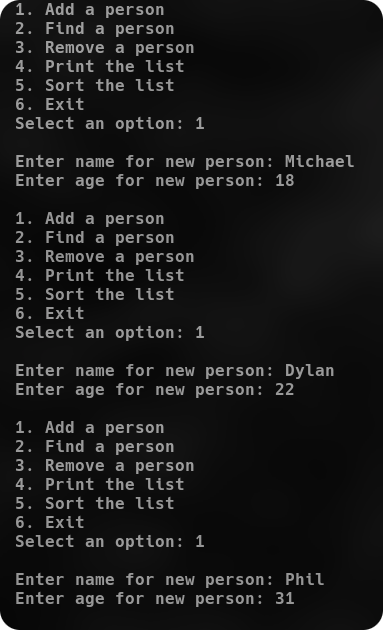
\includegraphics[width=.9\textwidth]{Figures/EC1.png}
  \caption{Extra Credit Test Run, part 1}
  \label{fig:1}
\end{figure}

\begin{figure}[H]
  \centering
  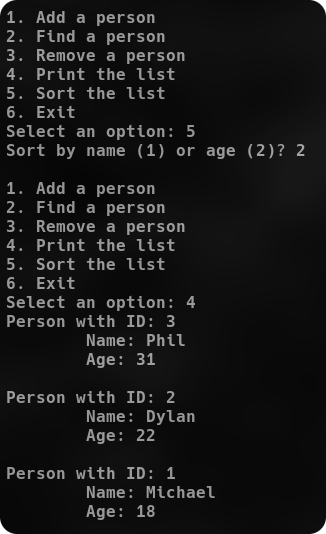
\includegraphics[width=.9\textwidth]{Figures/EC2.png}
  \caption{Extra Credit Test Run, part 2}
  \label{fig:2}
\end{figure}

\begin{figure}[H]
  \centering
  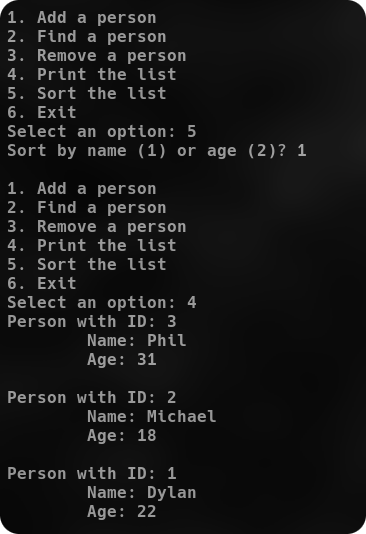
\includegraphics[width=.9\textwidth]{Figures/EC3.png}
  \caption{Extra Credit Test Run, part 3}
  \label{fig:3}
\end{figure}

\section{Conclusion}

Overall, due to the heavy reliance on knowledge of pointers, memory address references, linked lists, class structures, and the ability to interface with the aforementioned, the lab provided an effectively advanced lesson regarding these concepts. Especially in terms of linked lists, working with them in an actual example allowed for a deeper understanding.

\section{Appendix}

\lstinputlisting[
    caption=Complete Source Code, % Caption above the listing
    label=lst:L6, % Label for referencing this listing
    language=C++, % Use C++ functions/syntax highlighting
    frame=single, % Frame around the code listing
    showstringspaces=false, % Don't put marks in string spaces
    numbers=left, % Line numbers on left
    numberstyle=\tiny, % Line numbers styling
    backgroundcolor=\color{black!5}, % Set background color
    keywordstyle=\color{magenta!80}, % Set keyword color
    commentstyle=\color{blue!80}, % Set comment color
    stringstyle=\color{green!80}, % Set string color
    breaklines=true
  ]{Code/personList.cpp}

\end{document}
